


\chapter{
 2012: A Spatial Capture-Recapture Odyssey
 }

\markboth{The End}{}
\label{chapt.final}

\vspace{0.3cm}


\vspace{2in}

Capture recapture methods have been a cornerstone of ecological
modeling and analysis for decades.  Yet there are essentially no real
capture-recapture data sets that come {\it without} auxiliary spatial
information about location of capture (but sometimes such information
is discarded).  As such, classical capture-recapture
models are usually not the right tool for the job of analyzing real
data sets, unless you happen to study fish living in a tank.
       % XXXX I would tone this down and say that "virtually all
           % classical analyses can be improved by making use of the
           % available spatial data.
Instead, biologists need methods -- spatial
capture-recapture methods -- that make use of spatial
information in their capture-recapture data sets.

Spatial capture-recapture methods resolve the essential problem of
capture-recapture, that of estimating population size,
and density 
but, by
explicitly linking space occupied by individuals with the spatial
location or region of sampling, they do so in a manner that provides a
holistic framework for answering ecological questions related to the
spatial structure of populations -- movement, space usage, spatial
variation in density, landscape connectivity, and other things.
 Thus, spatial capture-recapture methods enable ecologists
to integrate science with their capture-recapture models based on
individual level encounter data.

In this book we summarized, synthesized and extended recent
developments of spatial capture-recapture models.  The ``big idea'',
if you could distill the whole thing into one idea, is based on the
 idea of extending closed population models by augmneting them with a
 point process model that describes the distribution of indivdiausl \citep{efford:2004} in
 space. As a conceptual matter then, the underlying point locations
 are regarded as an individual covariate in the encounter part of the
 capture-recapture model. In a sense, thats really all there is too
 it. But the relevance is much bigger and more profound because, once
 we have made space explicit in the model, then we can think about
 building explicit spatial models.
We talked about some ideas: landscape connectivity, resource
selection, modeling spatial variation in density. These are all by
themselves profound extensions of the basic capture-recapture method
and it broadens and expands the relevance and utility of
capture-recapture for studying animal populations.  
There remains much to be done in the continued development of SCR
models. In the following section, we make light some topics that we
think are suggested by existing ideas or that we talked about briefly
in the book but need further development. Some of these would make
idea graduate projects or similar.


\section{The Growth of Spatial Capture-Recapture}
\begin{comment}
Everyone in ecology is familiar with the method of species
distribution modeling known as MaxEnt \citep{phillips_etal:2006}. 
I did a google search on ``MAXENT'' AND ``species distribution''

since 2002  2140 cites
since 2003  2140 cites
since 2004  2140 cites
since 2005  2130 cites  10 published in 2004
since 2006  2120 cites  10 published in 2005
since 2007  2090 cites  30 published in 2006
since 2008  2010 cites  80 published in 2007
since 2009  1840 cites 170 published in 2008
since 2010  1580 cites 260 published in 2009
since 2011  1220 cites 360 published in 2010
since 2012   743 cites 477 published in 2011
since 2013   118 cites 625 published in 2012 
                       118 published in 2013 so far
\end{comment}


On March 6, 2013, 
we did this Google Scholar search:
\begin{verbatim}
 ``spatial capture recapture'' OR ``spatially explicit capture recapture''
\end{verbatim}
The results are described here and, we think, suggest a bright future
for the development and application of spatial capture-recapture
models.  Most (but not all) of these papers are about the type of SCR models
discussed in this book although a handful had to
do with other types of spatial analysis as related to
capture-recapture models.
The results from this literature search are shown
in tabular form in Tab. XXX. 
\begin{verbatim}
since 2002   274 cites
since 2003   274 cites 0 articles
since 2004   271 cites 3 articles published in 2003
since 2005   269 cites 2 articles published in 2004  Efford 2004
since 2006   264 cites 5 articles
since 2007   261 cites 3 articles
since 2008   253 cites 8 articles Borchers and Efford and Royle 
since 2009   242 cites 11 articles
since 2010   222 cites 20 articles
since 2011   176 cites 46 articles
since 2012   111 cites 65 articles
since 2013    27 cites 84 articles published in 2012
                       27 so far since March 6
\end{verbatim}

We see rapid growth in the number of citations. Somewhere in 2003 the
first relevant article was published (this was \citet{parmenter_etal:2003})
and there was subsequent growth fueled by publication of
\citet{efford:2004} and the release of the software DENSITY
\citep{efford_etal:2004}. In 2012 there were 84 articles published and
27 through the first 9 weeks of 2013.

Considering the number of citations as an ordinary population (without
spatial context!), we used these data to make a projection of the
number of published articles that involve SCR methods into the future.
We fitted an exponential growth curve to these data and estimate the
annual rate of growth to be 33.4\%, accounting for the partial year of
data observed in 2013.  We used the model to project the number of
publications that involve SCR models into the future
(Fig. \ref{last.fig.expgrowth}). This includes the observed data
(solid circles) (omitting the partial year 2013) and projections up to
2020.  We conclude that the future of SCR is bright, with 800 or 900
publications predicted to occur in 2020. While this is a long time in
the future to be predicting based on an exponential growth model, we
can do some model checking along the way, as the prediction of 85 SCR
publications in 2013 and 119 in 2014 can be assessed in short order,
giving us some short-term feed-back on the state of the system.  Of
course, this model is missing some important things. One of those is
carrying capacity. The model predicts $>800$ publications in 2020, but
there may not be that much capacity to do capture-recapture studies!




\begin{figure}[ht]
\centering
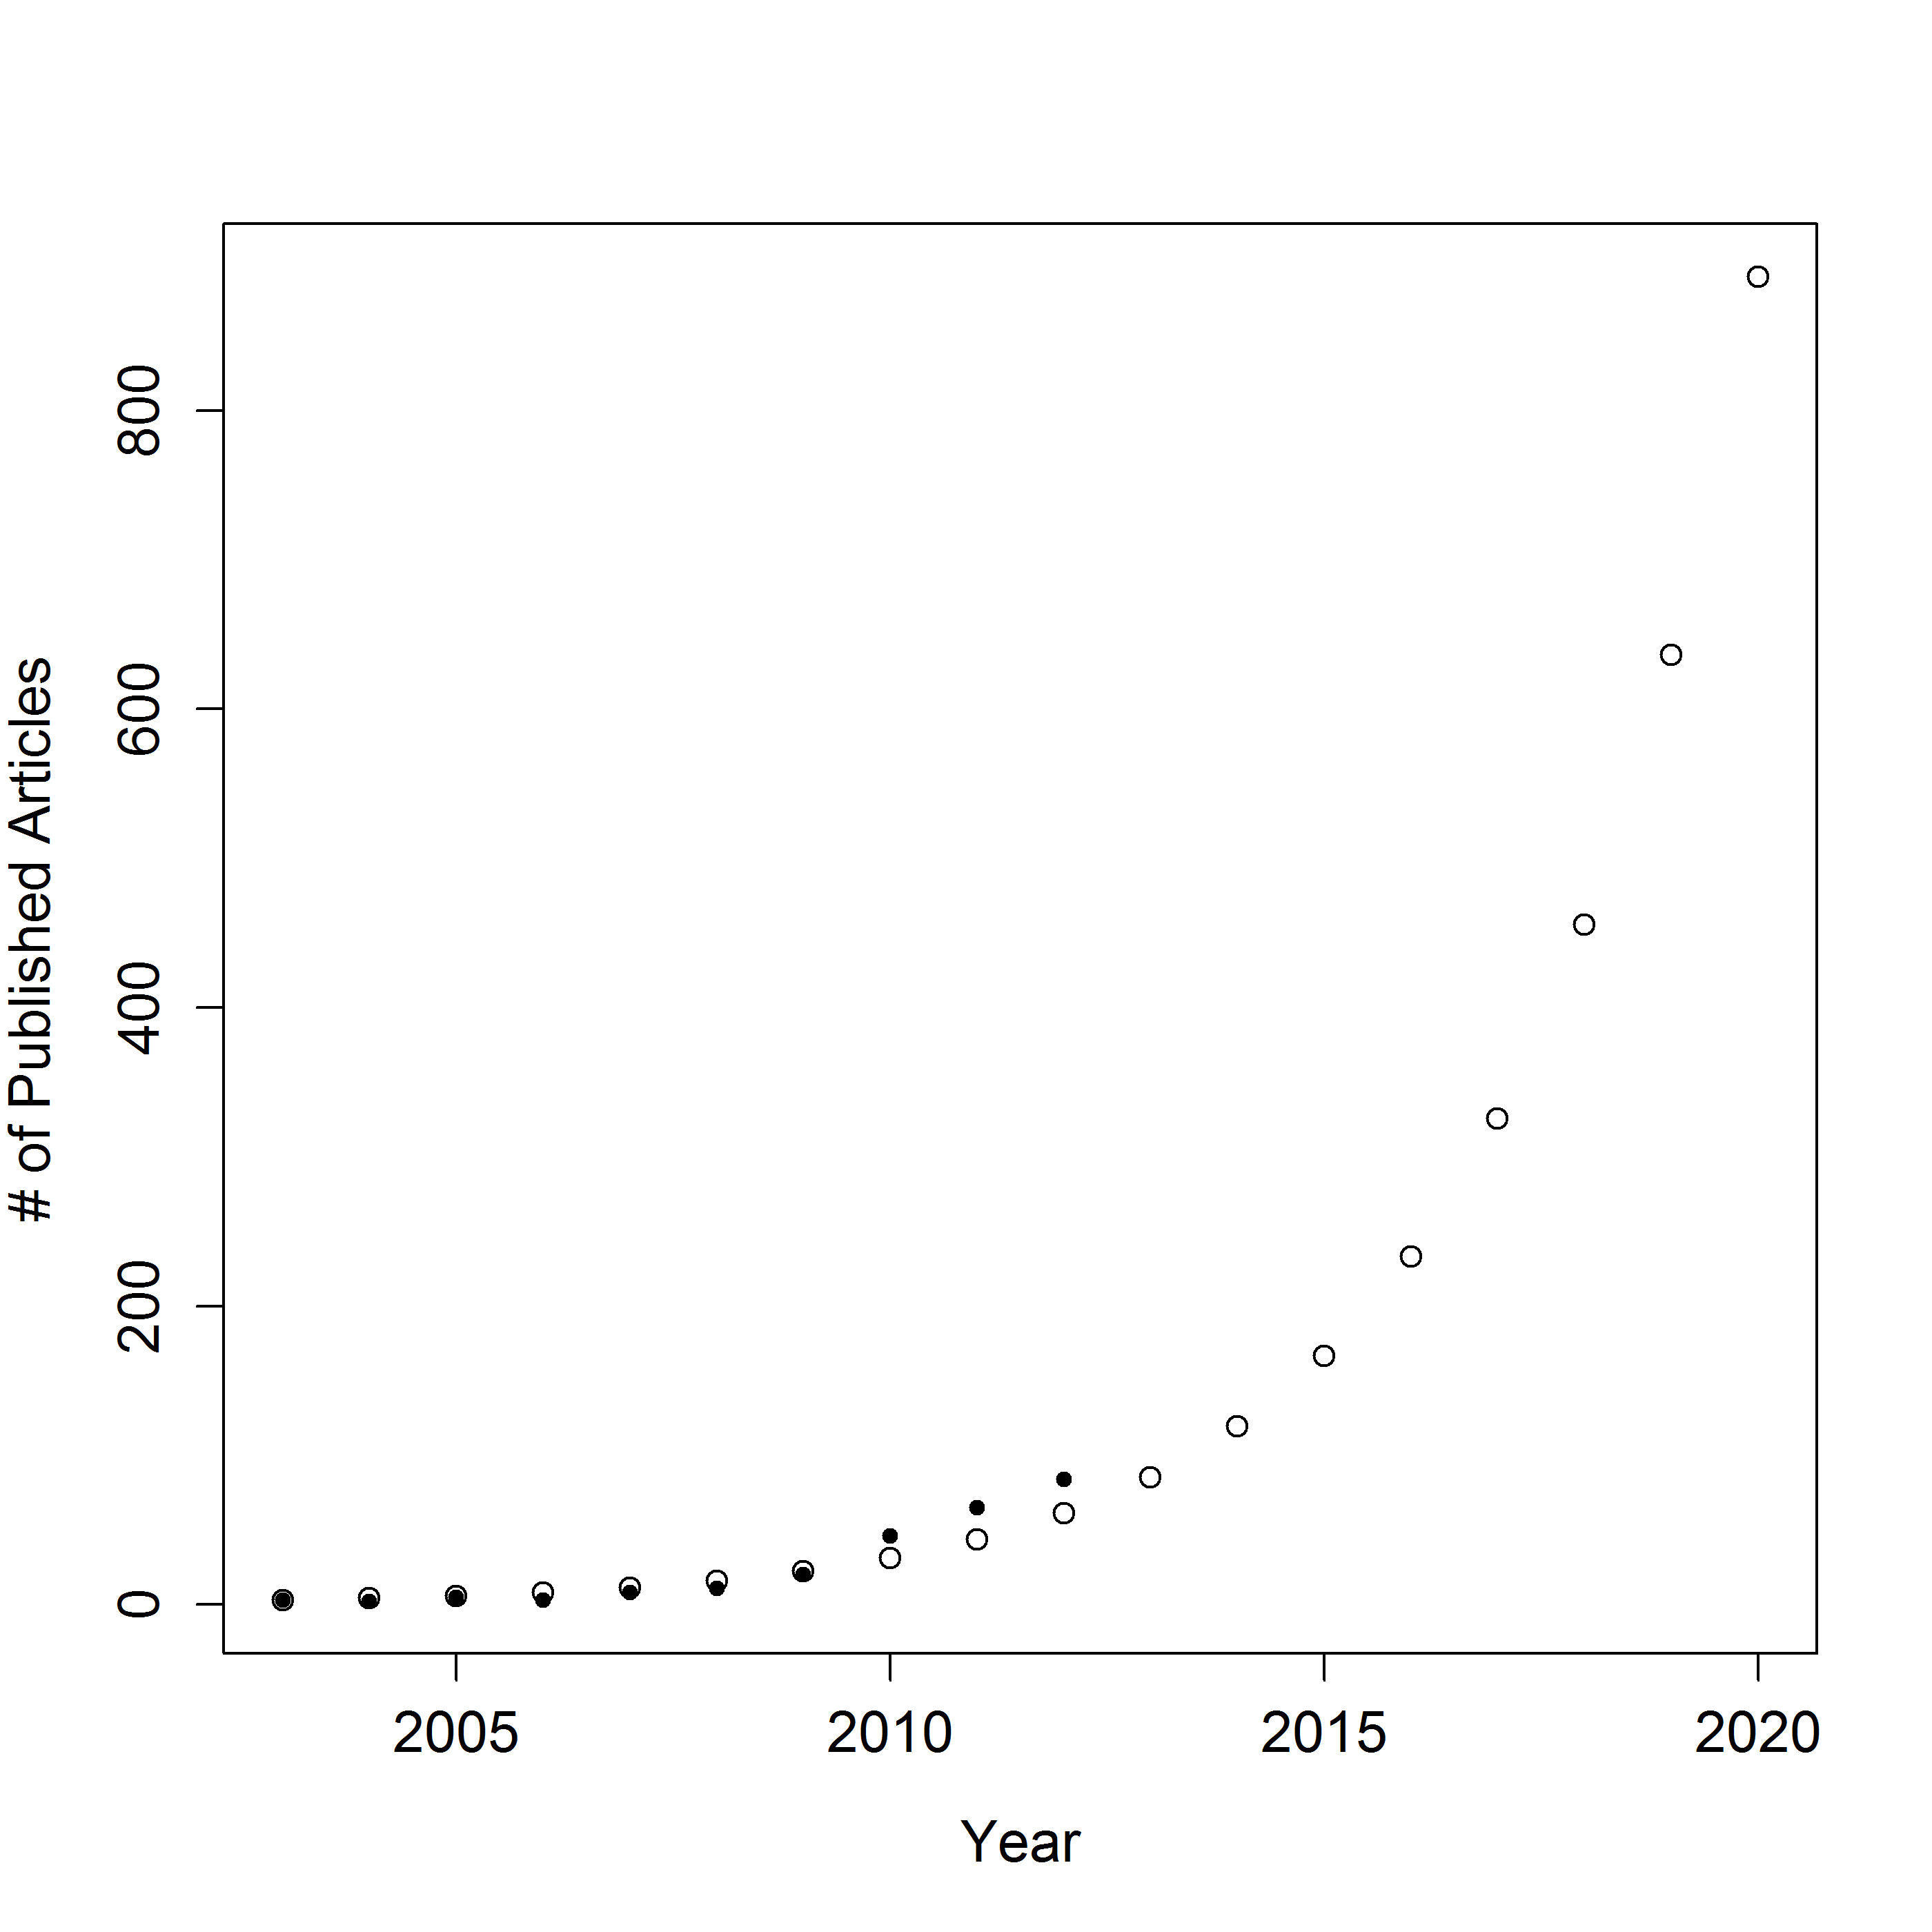
\includegraphics[width=4in,height=4in]{Ch20-Last/exp_growth.png}
\caption{
exponential growth projection of population size of published articles
that involve SCR models. 
}
\label{last.fig.expgrowth}
\end{figure}



\section{Emerging Topics}


In this book, 
we provided an overview and synthesis of capture-recapture methods as
known to
us 
around the end of 2012. There 
are many emerging topics which we have not covered either because lack
of technical knowledge, or satisfactory development, or no good
framework for implementation.

A number of topics of importance, or that people are working on, or
that might make good PhD or Masters projects.


\subsection{Inhomogeneous Point Processes}

In currently developing work, we (including Brian Reich, NCSU) propose a model that accounts for
spatial variation in home range density and potential interactions
between individuals' home ranges.  This model lets the activity
centers follow an inhomogeneous Strauss process
\citep{strauss:1975}, which allows for spatial variation
in the home range intensity, and includes a parameter that determines
the strength of repulsion between home ranges. 
The development of this work includes a simulation study, 
where it was found that properly accounting for interactions between
individuals can provide a substantial improvement in estimating
population size.  And thus far, for simulated data generated with interaction, the
usual independence model has a significant bias for the population
size, and generally has larger uncertainty for the population size
than the proposed Strauss process model.

While the Strauss model is intuitive and shows great potential, it
presents computational challenges.  The first challenge is that 
the likelihood includes a
high-dimensional integral that has no closed form.  To address this
issue, we develop an approximation to the
Strauss likelihood which allows for posterior sampling, extending related
work for categorical Markov random fields
\citep{green:2002,smith:2006}.  The second challenge is that 
because $N$ is treated as an unknown
parameter to be updated and hence $N$
varies and so does the dimension of the likelihood, and thus the
posterior.  In this case, we can overcome this dimension-changing problem using an
auxiliary variable scheme in the Markov chain Monte Carlo algorithm.
While the results from an initial analysis of simulated data verifies that this computational
approach leads to reliable inference, there are still many areas to be explored in
using the Strauss model and other models of clustering.


\subsection{Combining data from different surveys}

In some instances, researchers apply different survey techniques to
the population of interest, because they yield complementary
information. For example, Camera trapping is the prime tool for
estimating population size/density and other demographic parameters
for uniquely marked species; genetic surveys can yield additional
information on the genetic diversity and health of a population that
we cannot study using camera traps. At the same time, genetic surveys,
when samples are analyzed to the individual level, also yield spatial
capture recapture data (see Chapt. \ref{chapt.search-encounter}). In
this situation, we have two data sets at hand that carry information
on animal density, and we should be able to get more precise estimates
of density if we combine these two data sets into a single SCR model.

\citet{gopalaswamy_etal:2012mee} developed two approaches to combining
data from different survey types. In the first case, both surveys are
carried out at the same time, so that we can assume that they both
sample the same -- closed -- animal population, i.e., there are no
possible changes in population density between the two surveys. For
camera trapping and genetic surveys, we cannot match records of
individuals between the two data sets. As a consequence, in the
combined model there are two sets of $z_i$, say, $z^{C}_{i}$ for the
camera trap data and $z^{G}_{i}$ for the genetic survey data. But
defining a single state-space around both sets of survey locations, we
can define a single data augmentation parameter, $\psi$, that refers to
both these sets of $mathbf{z}$.  {\bf XXX ANDY; WE STILL HAVE TWO ESTIMATES
OF N AND THUS D; HOW DID YOU CHOOSE? OR DID YOU AVERAGE? I DONT FIND
ANY INFORMATION ON THAT IN ARJUNS MS XXXXX}

Further, since the scale parameter of the trap encounter model (in
\citet{gopalaswamy_etal:2012mee} the Gaussian model), $\sigma$, is
related to animal movement, we can expect this parameter to be the
same for both surveys and share it across both data sets. Finally, we
need to define separate baseline detection parameters, say
$\lambda_{0}^{C}$ and $\lambda_{0}^{G}$, because the processes
governing detection by the survey methods should be
different. \citet{gopalaswamy_etal:2012mee} found that this combined
model did indeed produce a more precise density estimate, compared to
single-data set models.  We can, of course, imagine other
parameterizations for this combined model -- we could specify both
$\psi$ or $\sigma$ as survey specific, if we have reason to believe
they changed between surveys, and we refer you to
\citet{gopalaswamy_etal:2012mee} for more details on these alternative
parameterizations.

A second approach of using information from one survey in the analysis
of a second survey (that maybe does not yield quite as much data as
the primary survey) is by analyzing your primary data set alone, then
taking the posterior distribution of a parameter both surveys share
and using it as an informative prior distribution in the analysis of
the second data set. \citet{gopalaswamy_etal:2012mee} refer to this as
the stepwise approach, and they implemented this approach by equating
the mean and variance of the posterior distribution of $\psi$ and
$\sigma$ from the photographic survey to the mean and variance of a
beta and a gamma prior for these parameters, respectively, for the
genetic survey. The authors found that this approach produced almost
identical density estimates compared to the combined model approach
described above.

In summary, no matter which approach is chosen, combining data across
surveys can help researchers to obtain more precise population
estimates, which is especially valuable when dealing with rare and
elusive species like big cats that almost always will produce sparse
individual data sets. Some thought has to go into the assumptions
underlying combining data -- for example, if there is a chance that
population size may have changed between surveys, it might not be
appropriate to have $\psi$ be a parameter shared across surveys; but
the assumption that $\sigma$ remains reasonably constant might still
be valid. The paper by \citet{gopalaswamy_etal:2012mee} considers the
situation where we have two SCR data sets, but we can imagine
combining SCR data with other sources of information, such as
telemetry data (see Chapt. \ref{chapt.partialID} and
Chapt. \ref{chapt.rsf} for examples), and possibly opportunistic
observations, although to our knowledge this latter issue has not been
tackled in the context of SCR, yet.


\subsection{Imperfect identification of individuals}

Imperfect identification of individuals can happen in a variety of
ways. In genetic surveys there is usually some probability of
mis-identification of individuals due to genotyping error
(e.g. \citet{lukacs_burnham:2005}). In camera trap survey a different
type of imperfect identification can occur when only the only one
flank of an animal is recorded in a detection event and that imagine
cannot be matched to any of the individuals identified by both
flanks. If that case, we can match single-flank pictures with the same
side flank pictures, but not with opposite side flank pictures and
thus cannot construct definite encounter histories for these
single-flank individuals (a right flank and a left flank picture could
be the same individual, or could be from two distinct
individuals. Finally, in Chapt. \ref{chapt.partialID}, in the context
of mark-resight models, we discussed the case where individuals can
either not definitely be identified as marked or not -- a violation of
a basic mark-resight assumption, and developed an approach to dealing
with the situation where we can always tell if an animal is marked or
not, but we are not always able to ascertain its individual identity.

In non-spatial capture recapture some efforts have been made to
formally deal with misidentification. \citet{stevick_etal:2001}
address this problem by double-sampling to derive an error rate for
genetic identification, and then including this error rate as a known
constant into a Lincoln-Petersen estimator of
abundance. \citet{lukacs_burnham:2005} develop an approach that
includes an additional parameter in the model -- the probability of a
genotype being identified correctly, which is estimated as part of the
model likelihood. \citet{link_etal:2010} developed an approach towards
solving the same problem implemented in a Bayesian framework that
relaxes some of the assumptions of the initial approach.
\citet{yoshizaki_etal:2009} deal with misidentification from camera
trap pictures due to evolving marks (i.e., natural marks that change
over time, such as scars). This situation is different from the
genotyping error one. Here, a change in marks creates a supposedly
`new' individual that can be recaptured several times, while the
original individual is never captured again (its mark is no longer in
the population). In contrast, in genotyping error it is assumed that
misidentification creates a `new' individual that is never observed
again, because each error leads to a new unique
genotype. \citet{yoshizaki_etal:2009} approach this situation
similarly, by including a parameter describing the probability of
correctly identifying an individual upon recapture (the parameter can
also be interpreted as the probability that a mark does not change
between capture occasions). Because of the dependencies between true
and false detection histories (when a `new' individual is created, the
`real' one can no longer be recaptured), the standard multinomial
approach to coming up with a model likelihood does not work and
implementing the model in a maximum likelihood framework is
difficult. The authors instead demonstrate an implementation of the
model based on minimizing a function of the squared differences
between the observed and expected frequencies of the observed capture
histories.

To our knowledge no attempts have been made to deal with
misidentification in an SCR framework. While all of the mis-ID cases
described above require distinct approaches, we believe that there is
one unifying theme to all of them: the location of the un or
potentially mis-identified records and the resulting probabilities of
belonging to certain individuals conditional on their activity
centers. For example, a right flank and a left flank camera trap
picture that are taken at two neighboring camera traps are more likely
to belong to the same individual that a right and a left flank picture
taken at cameras at opposing ends of the trap array, especially if
animal movement is smaller than the extent of the trap array; an
unidentified record of a marked individual in a mark-resight survey is
more likely to belong to a marked individual whose activity center is
close by, than to an individual whose activity center is located far
away; and so forth. Formally developing misidentification models
should be a focus for future SCR model development.

\begin{comment}
\subsection{Three dimensional space}

Throughout this book we have treated space as
two-dimensional, meaning that activity centers are assumed to occur on
the real plane. This approximation of reality is reasonable for many
terrestrial species, but aquatic organisms, especially marine animals
move about in three-dimensional space. Treating space as
three-dimensional could also conceivably be useful in studies of
flying organisms, aquatic organisms,
or species that use multiple strata of tall forests; however, we
suspect that two dimensional models of space should suffice in such
contexts. Regardless, a three-dimensional view of space requires that
activity centers $\bf s_i$ are indexed by
$x,y,z$ coordinates. In theory, this presents no problem whatsoever. In
practice, estimation based on integrated likelihood methods must
involve a three-dimensional integration. This will clearly be more
computationally demanding, but it should be possible using packages
such as {\tt R2Cuba}.
\end{comment}

\subsection{Gregarious species}

One of the key assumptions of the SCR models that we described
throughout this book is that the activity centers are independent of
one another.  There are good biological reasons why this shouldn't be
the case, and one of those is when species associate with one another
as a pair, or family group.
 Even species regarded as solitary often join family
groups for some portion of their life cycle.  We believe that general
models for non-independence of activity centers can be developed (see
item XXXX above) 


There are two consequences of individuals that exist as a pair or
group. For one, the detections are not independent. A trap that
catches one of the individuals is likely to capture others in the
group (Russell talked about this at TWS). The other consequence is
that the activity centers ${\bf s}_{i}$ should appear clustered or, in
fact, completely redundant in some cases. 
A possible way to account for this 
is to change our definition of ${\bf s}_i$ from the
location of an individual's activity center, to the location of a
group's activity center. We then expand our model to include a
submodel for group size, and we can estimate both the density of group
activity centers and total population size.



\subsection{Design}

model-based design is huge. Design of SCR studies is naturally
amenable to standard considerations of model-based spatial design
(BOOK XXXXXX) which we introduced back in
Chapt. \ref{chapt.design}. Clearly more work can be done on this
problem and we think at some point not too far into the future, there
will be general-purposes platforms for building capture-recapture
sampling plans. 
A number of specific design problems require some
investigation...... designing large landscape scale capture-recapture
studies where uniform coverage with traps cannot be achieved, needs
to be done.  
Design in the context of modeling spatial variation in
density..... and the effect on design of having telemetry or other
auxiliary data. 


\subsection{Borchers acoustic}

from ISEC

\subsection{Single Catch Traps}

In Chapt. \ref{chapt.poisson-mn} we talked about multinomial models in
which encounter of individuals is independent for all
individuals. this is 
the multi-catch type of device in which traps never fill-up, but an
individual can only be caught in one trap. 
We suggested (Following Efford XXXXX) that the multi-catch,
independent multinomial model, could be used for ``single catch''
traps (traps that hold a single individual or ``fill up'')......

A formal model for this situation is needed...........

\subsection{Model Fit and Selection}

Evaluation of model adequacy or ``fit'' is an important part of any
applied analysis. In Chapt. \ref{chapt.gof}, we offered up a number of
ideas based on standard considerations and applied them to SCR
models.  However, these ideas have not been widely applied, or evaluated, and much
work needs to be done. In particular, some basic analysis of their
power under meaningful alternatives would increase their relevance and
possibly lead to insights for devising better methods. This applies to
both Bayesian and likelihood-based methods, for which there are even
fewer published applications of fit assessment.

Similarly, we discussed model selection strategies using more-or-less
conventional ideas based on AIC/DIC, and model indicator
variables. Calibration of these methods under alternatives is needed,
along with 
some analysis of sensitivity to density estimates to misspecification
of certain model components.



\subsection{Dynamics}

Dynamic point processes:
Movement, Dispersal, Migration
Transience.


\subsection{Misc. Topics}

Models for unmarked or partially marked individuals integrated with RSF data from telemetry

Occupancy and counts data + SCR data (AOAS and Sollmann et al.)

Spatial genetics  -- can use SCR to study gene flow, related things....

SCR on dendritic networks (streams and trails).





\section{The Future of SCR}

Everything in ecology is spatial, and now so too are capture-recapture
models.

Historically the main use of capture-recapture was to obtain population
size estimates, but
SCR models allow you to address basic and applied questions of
population ecology from individual encounter history data. Problems
having to do with movement, space usage, landscape connectivity, and
how individuals organize themselves in space. 

We envision that SCR models will be useful in helping
ecologists ``do science'' by developing explicit models of spatial
processes, space usage, connectivity, etc., using ordinary, cheap, and
easy to obtain individual encounter history data. Much work needs to
be done to improve computational feasiability, to address many
technical or methodological holes in the literature (see previous
sections), and to make these methods accessible to practiioners.











